\documentclass[11pt]{article}
\usepackage[top=1.00in, bottom=1.0in, left=1in, right=1in]{geometry}
\renewcommand{\baselinestretch}{1.1}
\usepackage{graphicx}
\usepackage{natbib}
\usepackage{amsmath}

\begin{document}
\bibliographystyle{/Users/Lizzie/Documents/EndnoteRelated/Bibtex/styles/besjournals}
\renewcommand{\refname}{\CHead{}}

\hspace{-5ex} \includegraphics[width=0.5\textwidth]{/Users/Lizzie/Documents/Professional/images/letterhead/ubc/Faculty of forestry.png}
\pagenumbering{gobble}
\vspace{1.5ex}\\

\setlength{\parindent}{0pt}
\setlength{\parskip}{7pt}
\today

Dear Dr. Rudolf:

We would be grateful for your consideration of our manuscript, ``A four-step Bayesian workflow for improving ecological science,'' as an Inspiring Perspective in \emph{The American Naturalist}. % ... and show how it can enhance data collection, forecasting, and statistical training.  % The workflow is designed to be broadly generalizable and practical. To make sure the steps are clear and accessible we would present full example of the workflow and accompanying code (in R Markdown) to estimate trends over time in plant and animal phenology. 

Given the increasing aims of forecasting and prediction today, ecologists are using more complex models to leverage larger datasets \citep{anderson2021trends,muff2022rewriting}. Many researchers---ourselves included---were not trained in best statistical practice for these approaches, which can lead to poor models and incorrect predictions and decisions. % However, while many ecologists may not be formally trained in the fitting of large, complex models, they often have the computational toolkit to approach such models, but lack an organizational framework to develop, test and improve bespoke models. 

To address this pressing gap, we outline a generalizable workflow \citep{grinsztajn2021,vandeschoot2021}, which is built on fundamental scientific principles and new insights from statistics and data science. This approach  moves away from a focus on null hypothesis testing, towards estimating effect sizes, using models calibrated and better understood through simulating data at multiple steps---using a number of skills more often associated with theoretical than empirical ecology. We conclude by highlighting how adopting this workflow has changed our science and how it may improve statistical and mathematical training in ecology. 

% Fitting larger and sometimes more complex models presents challenges that can be overcome by approaching analyses through specific workflows \citep{betanworkflow,grinsztajn2021,vandeschoot2021}, which themselves are built on a process of how to do not just statistics, but how to do science \citep{box1976science}. Such approaches move away from a focus on null hypothesis testing, towards estimating effect sizes, using models calibrated and better understood through simulating data at multiple steps---using a number of skills often reserved in ecology more for `theorists' than empirical ecologists. But this theoretical-vs-empirical divide ignores that the average modern ecologist is computational, and thus already has many of the basic skills to build bespoke models. 
% We then outline one such iterative workflow, which contains four steps (see Fig. \ref{fig:workflow} below), highlighting how it has changed our science and how it may alter statistical and mathematical training in ecology. These steps include discussion (and definitions) of model calibration, non-identifiability, prior predictive checks, power analyses through simulation and iterative model building. 

% The manuscript is authored by an international and interdisciplinary group of ecologists, evolutionary biologists and statisticians. The workflow follows the basics of how authors EM Wolkovich, TJ Davies and WD Pearse approach model building and leverages the insights and skills of computational statistician M Betancourt who has developed fundamental statistical workflows for diverse scientific disciplines. We have designed it to be broadly generalizable and practical, including relevant examples of forecasting shifts in animals and plants over time.

{\bf We have included previous reviews of this manuscript} from \emph{Nature Ecology \& Evolution}. In response to these reviews we have made a number of changes to the manuscript, including clarifying its scope and goals, providing a GitHub repository (not shown here for double-blind review) and shortened the manuscript (2700 words currently) so that it is accessible for more readers. We would be happy to detail these changes further if requested. 

We hope that you will find this perspective, which provides a road-map for the many ecologists now building more complex models, suitable for publication in \emph{The American Naturalist}. %By integrating simulation more fully in model building and testing this workflow can fit models that are more robust and well-suited to provide new ecological insights. % This manuscript is not under consideration elsewhere, and all authors approved of this version for submission. 

Sincerely,\\

\includegraphics[scale=1]{/Users/Lizzie/Documents/Professional/Vitas/Signatures/SignatureLizzieSm.png} \\

Elizabeth M Wolkovich\\
Associate Professor of Forest \& Conservation Sciences\\ 
University of British Columbia\\

\newpage
{\bf References}
\vspace{-8ex}
\bibliography{..//refs/bayesrefsmini.bib}



\end{document}

\newpage
{\bf Example figures}


\begin{figure}[ht]
\centering
\noindent 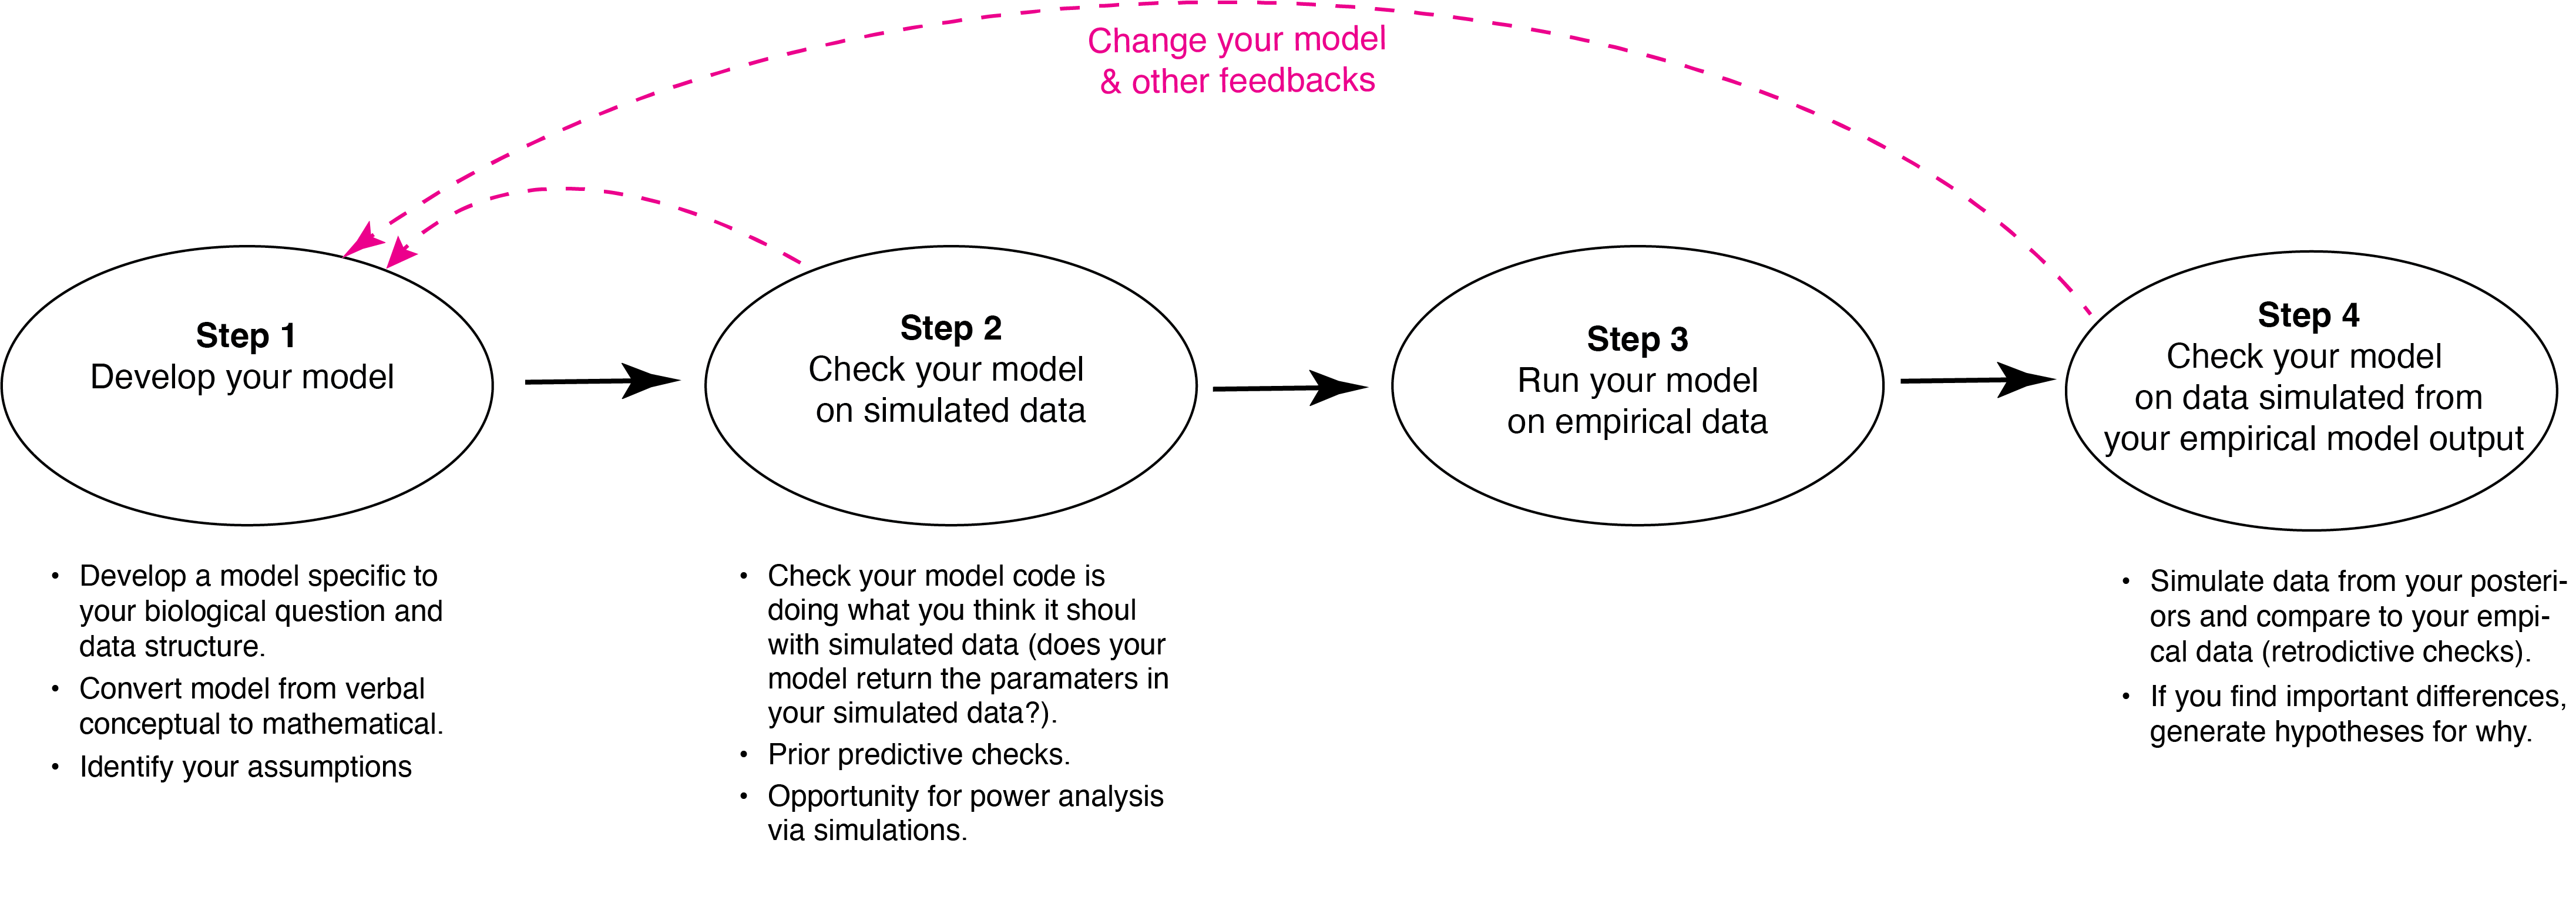
\includegraphics[width=1\textwidth]{..//figures/workflow.png}
\caption{The four-step iterative workflow we outline can help design models for specific ecological questions, data and aims---which makes this a statistical workflow that can naturally become a scientific workflow. It makes the step that many of us focus on---running your model on your empirical data (Step 3)---far more straightforward and insightful by using simulations both before (Step 2) and after (Step 4) it to better understand the model and data together.}
\label{fig:workflow}
\end{figure}

\begin{figure}[ht]
\centering
\noindent 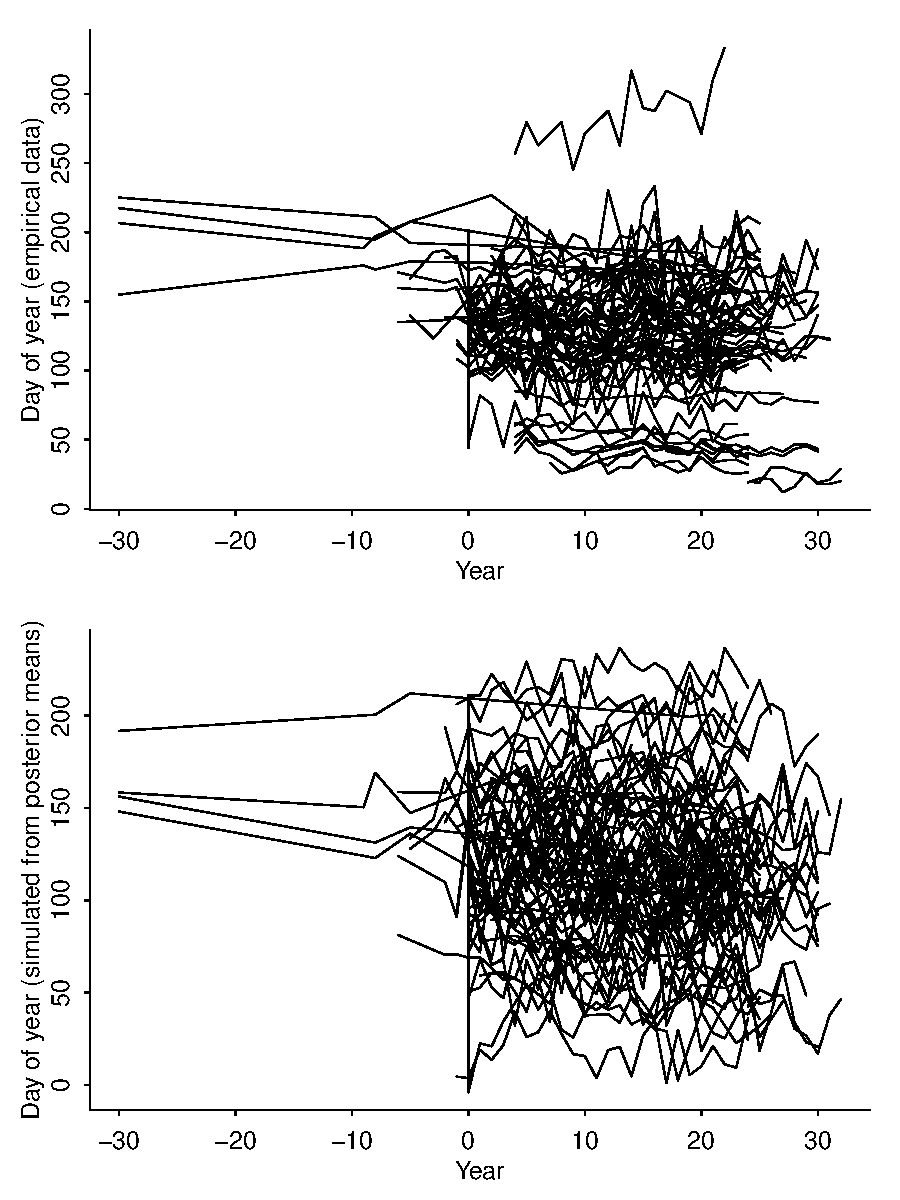
\includegraphics[width=0.6\textwidth]{..//examples/synchrony/graphs/rawvsonepredictivecheck.pdf}
\caption{Example of a single retrodictive check from time-series data of phenological events over time. The raw data (top, black) looks similar to one simulated dataset (bottom, purple), based on existing species number, their respective $x$ data, and simulating from the parameters for each species. See `An example workflow' in the Supplement for more details.}
\label{fig:retrodictivecheck}
\end{figure}


%%%
%%%

\begin{figure}[ht]
\centering
\noindent 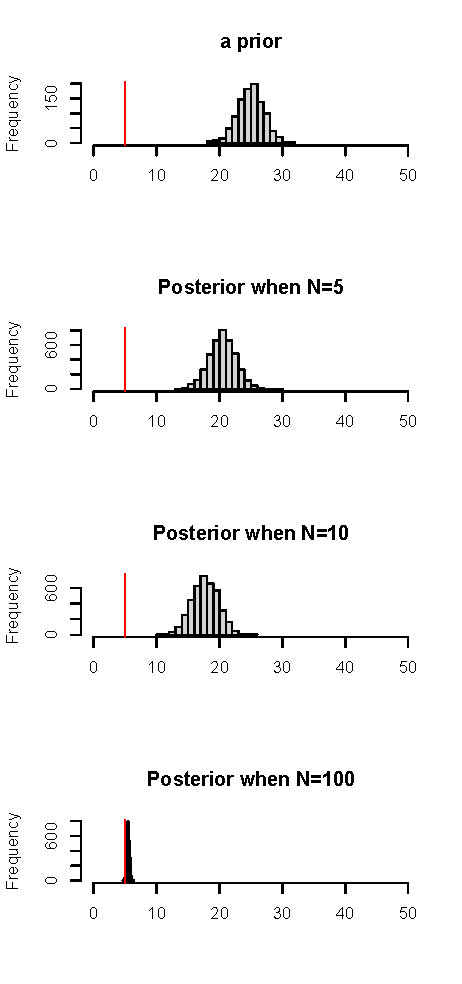
\includegraphics[width=0.5\textwidth]{..//examples/misspecifiedmodel/priorpostforflows.pdf}
\caption{A simple example of how to use simulated data to understand calibration issues in a mis-specified model. Here we know the true model underlying the data is $y=\alpha + \text{normal}(0, \sigma)$ where $\alpha$ is 5 (shown as blue vertical line) and $\sigma$ is 2. The model, however, is mis-specified by a prior for $\alpha$ of $\text{normal}(25, 2)$ (dashed blue line), resulting in a posterior (salmon-colored histogram) not centered on the true value. In our experience it is quite rare to have a prior informed by ecological knowledge be so far off, but this is an example. How mis-calibrated the model will be depends on the data: we show examples with a sample size ($N$) of 5, 10 and 40 data points. In practice these studies would allow us to determine how much data we would need to be robust to suspect prior models. (Note the change in $y$ axis range for bottom plot.) }
\label{fig:misspecifyprior}
\end{figure}


